通常Serverless平台中,
用户部署代码后,
平台需要分配资源、下载代码(或者镜像)、
初始化、
启动实例等环节,
这些步骤都是比较耗时的操作。
而只有这些操作完成后,
实例才具有服务的能力,
这种延时称之为冷启动问题,
它决定了Serverless平台弹性伸缩的能力,
如\cref{cold_start}所示。

\begin{figure}[ht!]
    \centering
    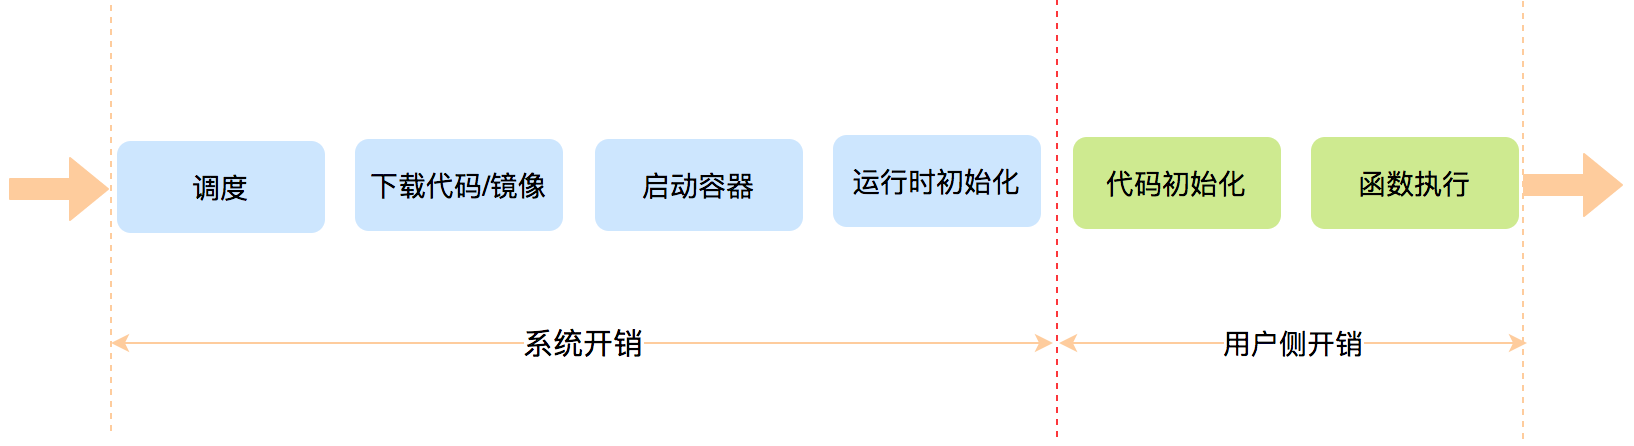
\includegraphics[width=\linewidth]{images/cold_start.png}
    \caption{冷启动的各个阶段\cite{meituan_serverless_nest}}
    \label{cold_start}
\end{figure}

\subsection{优化镜像加载时间}
镜像的加载是一个必须要考虑的问题,
常规的执行方式是在实例上下载代码,
或者需要下载用户自定义的镜像。
然而这些自定义的镜像可能非常大,
例如,
AWS Lambda支持最大250Mb的代码(Zip包),
或者大至10G的镜像。
优化初始化时间的常规做法有:

\begin{itemize}
    \item 裁减镜像或者使用轻量级虚拟化技术,
    提高镜像的启动速度\cite{meituan_serverless_nest, tecent_faas_cold_start},
    \item 对代码进行缓存以避免重复下载\cite{tecent_faas_cold_start}
    \item 优化运行时的加载速度,例如Java使用JIT\cite{carreira2021warm}
    \item 优化VPC网络以提高下载速度\cite{tecent_vpc_cold_start}
    \item 使用高效的压缩算法,例如使用Zstd压缩算法\cite{meituan_serverless_nest}
\end{itemize}

AWS Lambda通过优化镜像的底层存储,
更进一步提升了镜像的加载速度,
其核心思想是优化镜像在分布式文件系统中的布局,
最大程度进行复用,
如\cref{lambda_container_layer_chunk}所示。

\begin{figure}[ht!]
    \centering
    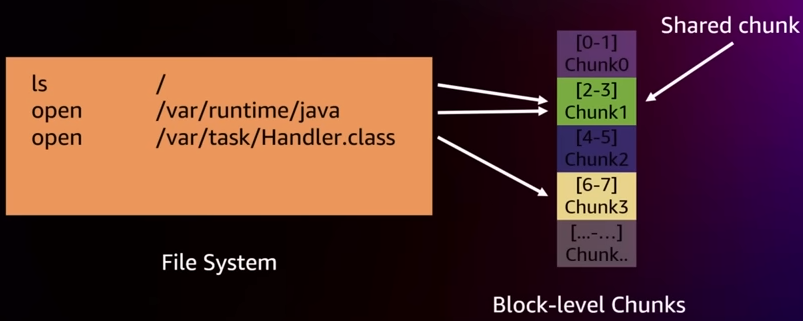
\includegraphics[width=\linewidth]{images/lambda_container_layer_chunk.png}
    \caption{AWS Lambda的镜像存储在分布式文件系统中的布局优化\cite{aws_lambda_2022}}
    \label{lambda_container_layer_chunk}
\end{figure}

\subsection{池化工作实例}
另一个解决冷启动的方式是提前创建工作实例,
阿里云、腾讯云等均支持预留实例,
允许用户预留一些实例\footnote{这并不是一个符合Serverless设计理念的做法,并可能因此产生额外的费用。}
根据流量情况进行实时预测,
利用一些算法进行预测(例如机器学习),
并按需进行自动扩缩容是普遍的实现
\cite{tecent_faas_cold_start,aws_lambda_2022,meituan_serverless_nest}。

工作实例创建完后,
如果流量下降,
一般也不会立即回收,
而是会采取一定的策略进行回收,
例如Azure Functions每20分钟回收一次\cite{aure_functions_cold_start}。
这样维护一个工作实例的池,
有助于降低平均的响应延迟。

\subsection{其他前沿的优化方案}
除了以上的一些常规策略外,
目前还有一些较为前沿的优化方案,
例如镜像快照、热容器等\cite{carreira2021warm, mohan2019agile}。
AWS Lambda已经上线了镜像快照,
将Lambda运行镜像的构建流程从函数调用触发前移到发布过程,
大幅降低了冷启动延迟,
如\cref{lambda_snapshot}所示。

\begin{figure}[ht!]
    \centering
    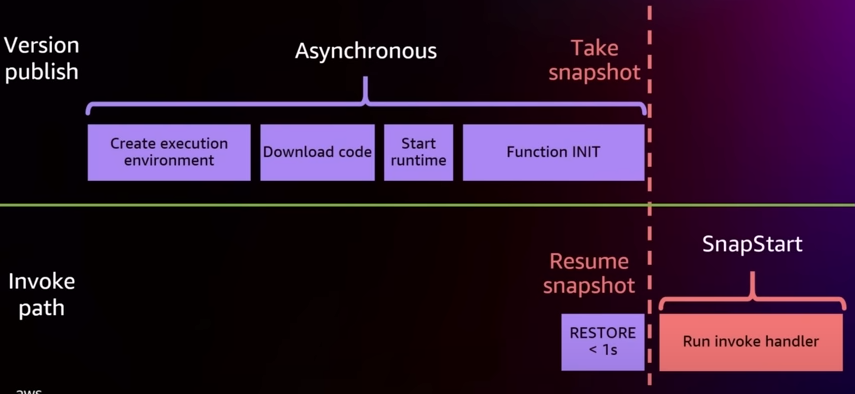
\includegraphics[width=\linewidth]{images/lambda_snapshot.png}
    \caption{AWS Lambda的镜像快照\cite{aws_lambda_2022}}
    \label{lambda_snapshot}
\end{figure}